\documentclass[12pt]{article}
\usepackage[colorlinks=true, linkcolor=blue, breaklinks=true]{hyperref} 
\usepackage{graphicx}
\usepackage{charter,amsmath,amssymb,breakurl}
\usepackage{eulervm}
\usepackage[letterpaper,margin=1in]{geometry}
\usepackage{multicol}
\everymath{\displaystyle}
\author{}\date{Due in class Friday 13 February}
\title{Math 104 Written Assignment 3}\author{}
\begin{document}
\maketitle
\pagestyle{empty}

\begin{center}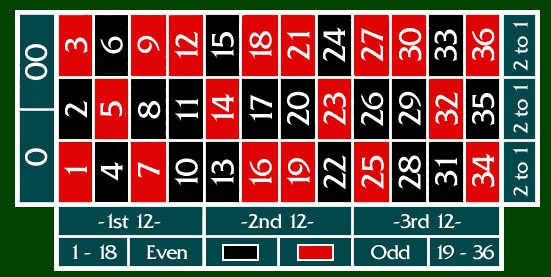
\includegraphics[scale=.3]{RouletteLayout}\end{center}
\begin{enumerate}
\item A {\em corner bet} is a roulette bet on any four numbers that form
a contiguous square on the roulette layout, which is shown above.
For example, a player could make a corner bet on the numbers
$\left\{1,2,4,5\right\}$.
\begin{enumerate}
\item Using the formula $\frac{36}{n}-1$ calculate the amount
the casino pays for a winning $\$1$ corner bet.
\vspace{1cm}
\item Calculate the probabilities of winning and losing a corner bet.
\vspace{1cm}
\item Calculate the expectation on a $\$1$~corner bet.
\vspace{1cm}
\end{enumerate}
\newpage

\item A {\em split} is a roulette bet on any two adjoining numbers
on the roulette layout.
For example, a player could bet on the numbers
$\left\{1,4\right\}$.
Another example of a split is $\left\{1,2\right\}$.
\begin{enumerate}
\item Calculate the amount the casino pays for a winning $\$1$ split.
\vspace{1cm}
\item Calculate the probabilities of winning and losing a split.
\vspace{1cm}
\item Calculate the expectation on a $\$1$~split.
\vspace{1cm}
\end{enumerate}

\item More generally, calculate the expectation
on a $\$1$ bet on any
$n$~numbers, where $n\le 36$ is any whole number.
\footnote{Of course, the $n$~numbers the player can
choose are subject to the rules of roulette, which in turn are determined
by the way the layout is arranged.}
\vspace{3cm}

\item The French roulette wheel has slots
labeled~1--36 and one slot labeled~0, but no
slot labeled~00 as in the US. However, the payoff
for a $\$1$~bet on $n$~numbers is still $\frac{36}{n}-1$
as in the US.
\begin{enumerate}
\item Calculate the expectation in France
on a $\$1$ bet on any
$n$~numbers, where $n\le 36$ is any whole number.
\vspace{1cm}
\item Is a roulette player better off playing in France
or in the US?
\vspace{1cm}
\end{enumerate}

\end{enumerate}
\end{document}
